\documentclass[11pt,a4paper,openany,oneside]{book}
\usepackage[utf8]{inputenc}
\usepackage[english]{babel}
\usepackage{amsmath}
\usepackage{color}
\usepackage{graphicx}
\usepackage{setspace}
\usepackage{amsthm}
\usepackage{amsfonts}
\usepackage{amssymb}
\usepackage{fancyhdr}
\newcommand*{\nesearrow}{\ensuremath{\searrow\mkern-18mu\nearrow}}
\newcommand{\virgolette}[1]{``#1''}
\usepackage{titlesec}
	\titleformat{\chapter}[display]
	{\normalfont\Large\bfseries}{\chaptertitlename\ \thechapter}{15pt}{\huge}
	\titleformat{\section}
	{\normalfont\large\bfseries}{\thesection}{1em}{}
\pagestyle{fancy}
\fancyhf{} % azzeriamo i campi
\renewcommand{\chaptermark}[1]{\markboth{#1}{}}
\renewcommand{\sectionmark}[1]{\markright{\thesection\ #1}}
\fancyhead[C]{\nouppercase{\leftmark}}
\fancyfoot[C]{\thepage}
\usepackage{subcaption}
\usepackage{cite}
\usepackage{url}

\usepackage[Sonny]{fncychap}

\ChNameVar{\Large}

\ChTitleVar{\Large\bfseries}




\theoremstyle{definition}
\newtheorem{defn}{Definizione}[chapter]
\begin{document}
	\thispagestyle{empty} 
	\begin{Large}
		\begin{center}
			UNIVERSIT\'A DEGLI STUDI DI PISA
		\end{center}
	\end{Large}
	\begin{figure}[!h]
	\centering
	
\includegraphics[scale=0.7]{fig/cherubino.png}
	\end{figure}
	\begin{Large}
		\begin{center}
			FACOLT\'A DI SCIENZE MATEMATICHE, FISICHE E NATURALI
			\vspace{1.5cm}

			%DIPARTIMENTO DI INFORMATICA
			%\vspace{0.1cm}

			MASTER DEGREE IN COMPUTER SCIENCE
			
			\textit{Data Science \& Technologies curriculum}
			%\vspace{1.5cm}
			%\textit{(classe L-31)}
			\vspace{2.5cm}

%			PROVA FINALE 
%			\vspace{1cm}

			\textbf{ReviewerNet.org:}


			\textbf{Visualizing Citation and Authorship Relations\\for Finding Reviewers}
			\vspace{1.5cm}
			\begin{table}[h!]
				\centering
				\label{my-label}
				\begin{tabular}{ccccc}
					Candidate              & {\color{white} aaaaaaaa} &  &  & Supervisors                 					\\Mario Leonardo Salinas &                                             &  &  						& Prof. Daniela Giorgi \\
				   &                                             &  &  &  Prof. Paolo Cignoni \\
				                           

				\end{tabular}
			\end{table}
		\end{center}
	\end{Large}
	\vspace{0.5cm}
	\begin{normalsize}
		\begin{center}
			Academic Year 2018 / 2019
		\end{center}
	\end{normalsize}	
\newpage
	\cleardoublepage
	\pagenumbering{arabic}
	\tableofcontents
	\begin{normalsize}
-----------------------------------------------------------------------------------------------
	\end{normalsize}
%	\textbf{Ringraziamenti}
%	\newline
	\textbf{Bibliography}
	
	\chapter{Introduction}\label{sec:introduction}
The number of digital academic documents, either newly published papers or documents resulting from digitization efforts, grows at a very fast pace: the Scopus digital repository counts more than 70 million documents and 16 million author profiles~\cite{scopus}; the Web of Science platform has more than 155 million records from over 34,000 journals~\cite{WoS}; Microsoft Academic collects about 210 million publications~\cite{MA}. In 2018, over four thousand new records were added to DBLP~\cite{DBLPrate}, and bibliometric analysts estimated a doubling of global scientific output roughly every nine years~\cite{BoMu15}. Therefore, the volume, variety and velocity of scholarly documents generated satisfies the big data definition, so that we can now talk of \emph{big scholarly data} \cite{KhLi17}. 

Sensemaking in this huge reservoir of data calls for platforms adding an element of automation to standard procedures -- such as literature search, expert finding, or collaborators discovery -- to reduce the time and effort spent by scholars and researchers. In particular, there has been an increase in the number of visual approaches supporting the analysis of scholarly data. Visualization techniques were proposed to help stakeholders to get a general understanding of sets of documents, to navigate them, and to find patterns in publications and citations. Federico et al.~\cite{FeHe17} survey about 109 visual approaches for analysing scientific literature and patents published in-between 1991 and 2016. Most of the works focused on the the visualization of document collections and citation networks. A more ambitious goal for visualization platforms would be to enable users get enough understanding to make decisions. 

In this work, we focus on the problem of reviewer finding by journal editors or International Program Committee (IPC) members, who are required to search for reviewers who know well a subject, yet are not conflicted with the authors of the paper under scrutiny. Finding good candidate reviewers requires to analyse topic coverage (possibly during time), stage of career, and past and ongoing collaborations. Every member of the community has its own approach to reviewer finding, which usually involves bibliographic research, and frequent visits to public repositories like DBLP~\cite{ley2002dblp} and researchers' home pages. In any case, one has to confront possibly large collections of data to make decisions, and a user may easily get lost after following a few links.  

We propose ReviewerNet, a visualization platform which facilitates the selection of reviewers. The intuition behind ReviewerNet is that the authors of relevant papers are good candidate reviewers. ReviewerNet offers an interactive visualization of multiple, coordinated views about papers and researchers that help assessing the expertise and conflict of interest of candidate reviewers.

\section{ReviewerNet in a nutshell}

\begin{figure*}[t]
\centering
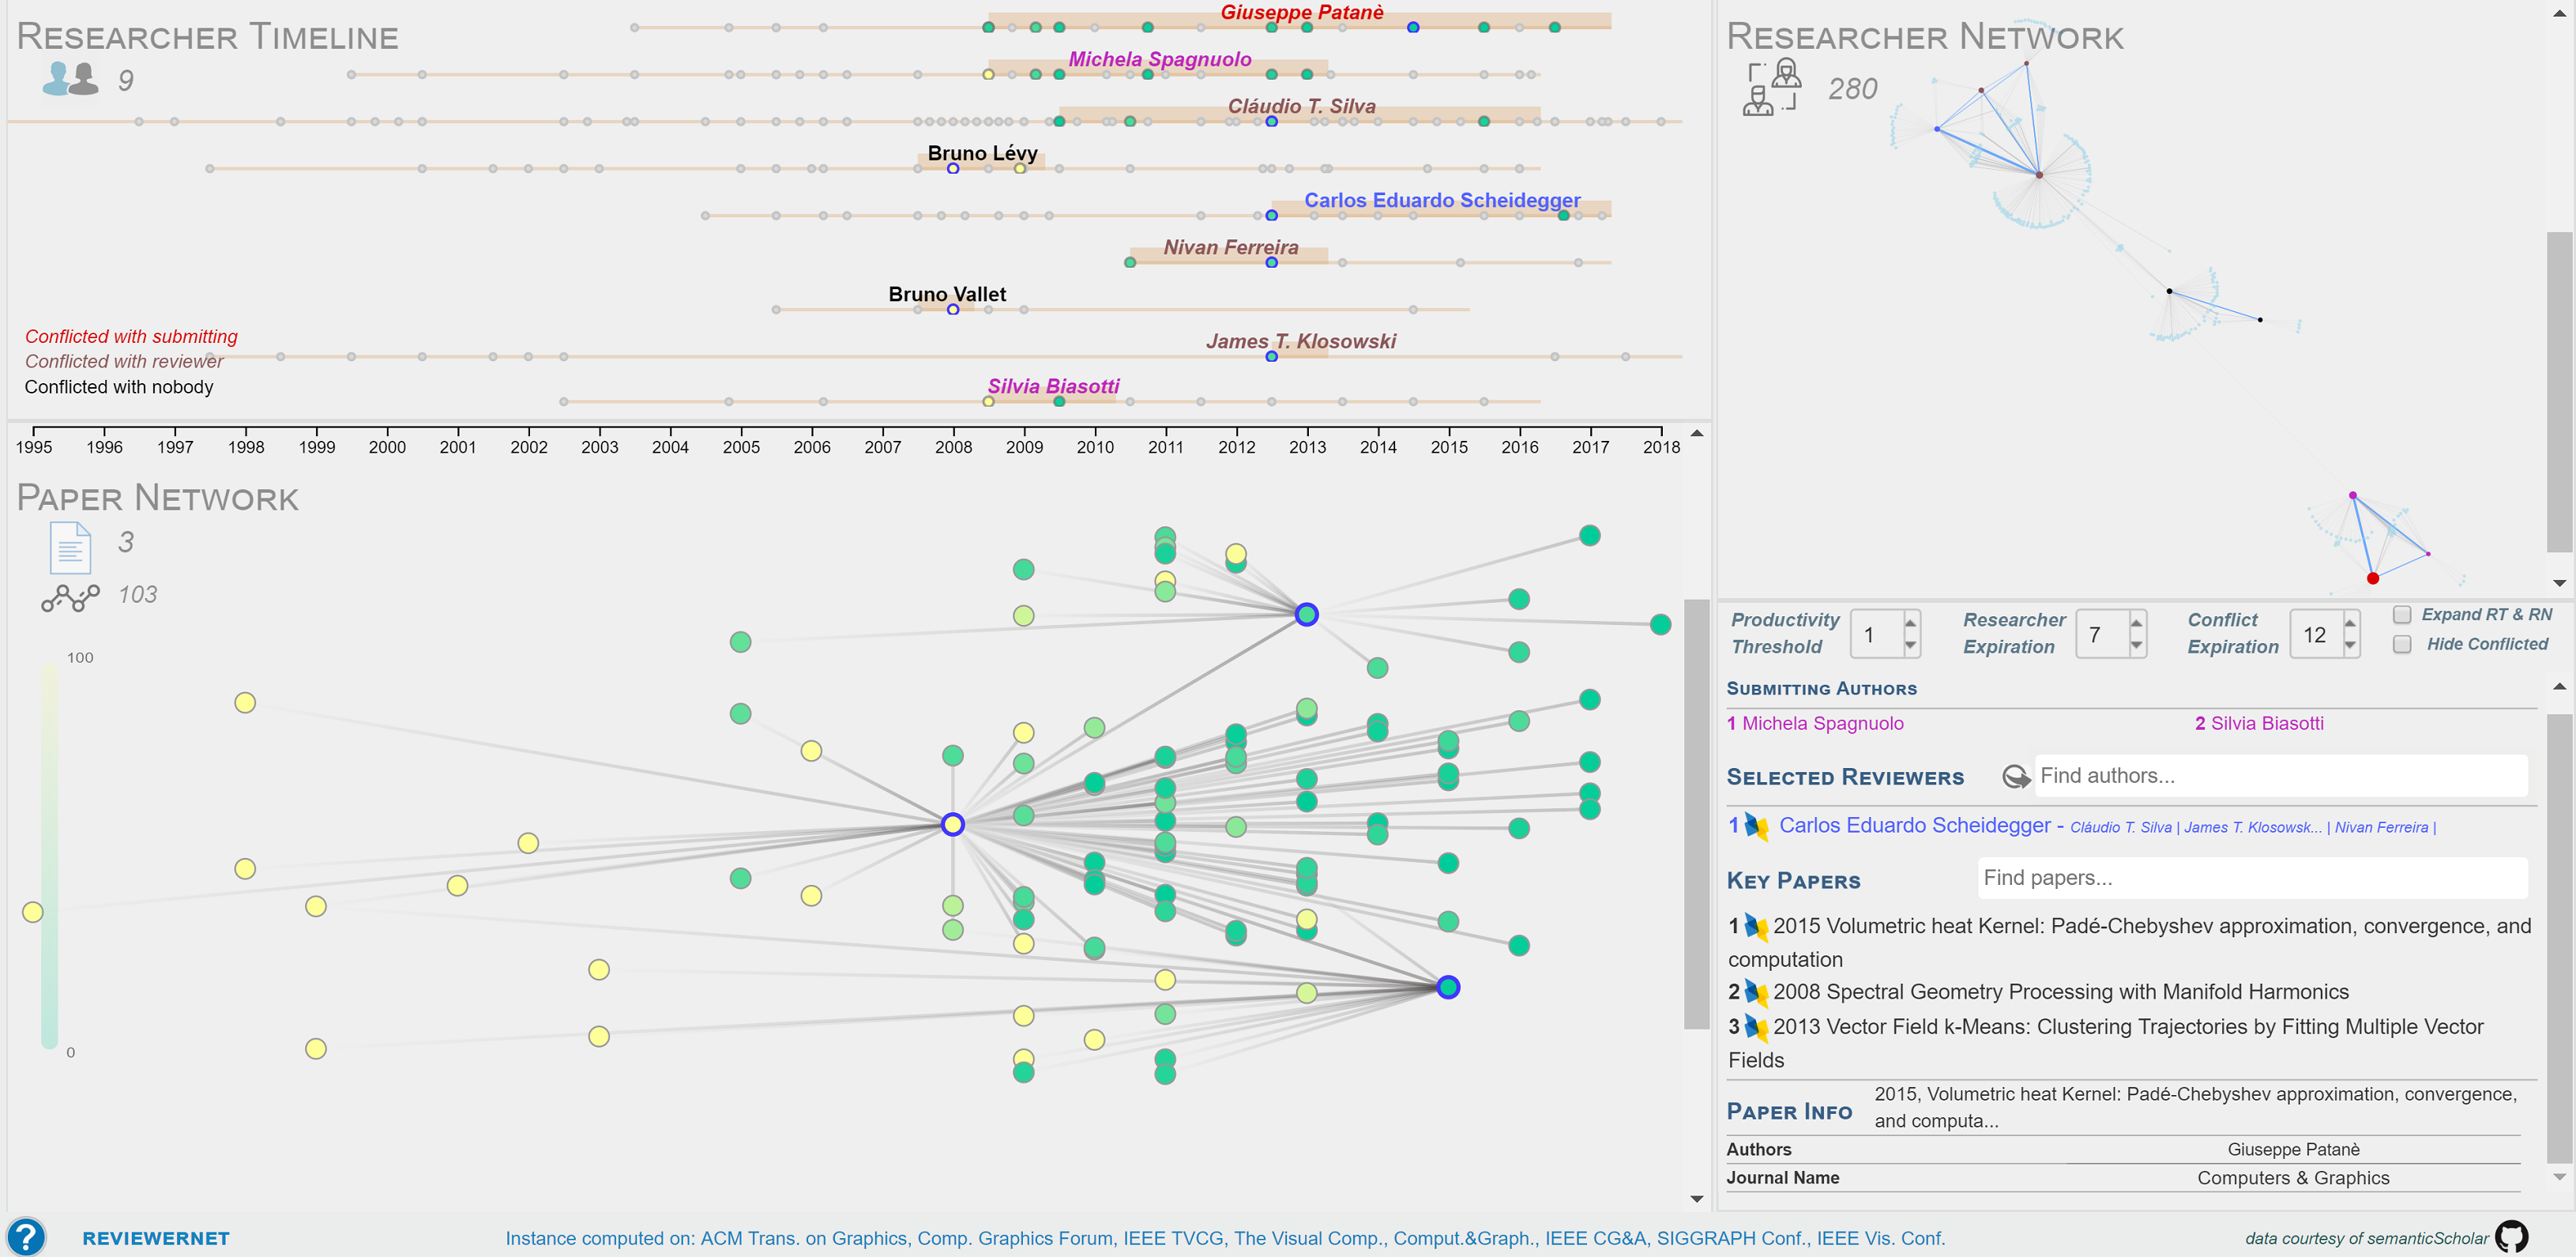
\includegraphics[width=\textwidth]{images/screenshot2.png}
\caption{The main interface of ReviewerNet, divided into four main areas: the \textsc{Researcher Timeline } (top left); the \textsc{Paper Network }(bottom left); the \textsc{Researcher Network } (top right); the \textsc{Control Panel } (bottom right). The interaction with these areas allows the users to identify researchers working on the topic defined by a network of papers, to analyse the researchers' contributions through time, and to get aware of co-authorship relations and conflicts.}
\label{fig:interface}
\end{figure*}

ReviewerNet supports the various actions that journal editors and IPC members perform while choosing reviewers, namely, searching the literature about the submission topic, looking for active experts in the field, and checking their conflict of interest. ReviewerNet does so by integrating an overview visualization of the literature with a visualization of the career of potential reviewers, their conflict of interests, and their nets of collaborators. This combined visualization helps to make sense of scholarly data, and rapidly get enough understanding to make a sensible decision, as shown in our user study (see Section~\ref{sec:evaluation}). 

ReviewerNet integrates the visualization of three main classes of data in a single window (see Figure~\ref{fig:interface}):

\begin{itemize}
\item  {\bf Paper Network} (PN): a chronologically ordered visualization of the literature citation network related with the submission topic. The nodes represent papers, while arcs represent in- and out-citation relations between papers. The horizontal dimension represents time. By means of interactive graph expansion functionalities, the PN supports the rapid exploration of key papers in the literature with respect to the topic of the submitted paper. The authors of the key papers identified will define the set of the candidate reviewers. The PN is built by the users, starting from a small number of seed papers of their choice;
\item  {\bf Researcher Timeline} (RT): a time-based visualization of the academic career of researchers, through horizontal lines and bars. The RT helps assessing the suitability of potential reviewers, showing thier topic coverage, productivity over years, and stage of career. Also, visual cues help the user to tell apart candidate reviewers from conflicting researchers. The RT is built automatically by ReviewerNet while the user builds the PN;
\item  {\bf Researcher Network} (RN), a graph visualization of co-authorship relations: the nodes represent the authors in the PN and their collaborators in the dataset; the arcs connect authors who have publications in common. The aim of the RN is to visualize the research communities: indeed, the identification of network of collaborators helps looking for sets of independent, non-conflicting reviewers. As with the RT, the RN is built online by ReviewerNet.
\end{itemize}
%
The basic pipeline for finding reviewers with ReviewerNet involves building the Paper Network starting from a small set of seed documents; evaluating possible choices of reviewers, by navigating the Reviewer Timeline and the Reviewer Network; and finally obtaining a justified list of chosen reviewers, along with possible substitutes suggested by ReviewerNet in case of decline.   

The user can navigate the different views and interact with the system through simple actions, to drive his/her investigation. Each view in ReviewerNet is linked to the other views, so that so that any action in a view is reflected in the others. Visual cues are used to improve the comprehension during interactive sessions: the colour, size, boundary, and style of visual elements visually represent important characteristics of the entities they stand for. Moreover, the coherence of visual cues across different views enforces their meaningfulness, and makes it easy for the user to switch between different views without losing focus.  

ReviewerNet builds on a reference database including papers, authors and citations from selected sources (journal articles and conference papers) taken from the Semantic Scholar Research Corpus~\cite{ammar:18}. ReviewerNet can be built over any dataset, according to the domain of interest.

\section{Summary of contribution}

We introduce the ReviewerNet visualization platform, which supports the reviewer selection process in the academic domain (Section~\ref{sec:methods}.

We describe and Section~\ref{sec:userinterface}). 

We demonstrate the platform in the field of Computer Graphics, with a reference dataset containing 17.754 papers, 108.155 citations, 23386 authors. We show how ReviewerNet can be used to search for reviewers who are expert on a certain topic, are at a certain career stage, who have a certain track of publishing records, who are not conflicting with neither the submitters nor other reviewers, and who are well-distributed in the scientific community (Section~\ref{sec:demonstration}). 

We evaluate the platform through a user study involving 15 real end-users from the Computer Graphics community, and show how they were able to get acquainted with ReviewerNet even with a very limited training, and how they rated very positively ReviewerNet functionalities (Section~\ref{sec:evaluation}).  

One of the main advantages of ReviewerNet is that it only relies on citations, to analyse the literature, and on co-authorship relations, to analyse conflicts. Citations are an essential part of research: they represent a credible source of information about topic similarity and intellectual influence. Moreover, since citations have author-chosen reliability, they are a very robust cue to relatedness. Similar reasonings hold for co-authorship relations. Therefore, an important contribution is the demonstration that a well-combined visualization based on citation and co-authorship relations only can support the reviewer search process, without the need for more complicated content analysis techniques.  

The tool is open, and the source code is available at~\url{https://github.com/cnr-isti-vclab/ReviewerNet}.  





	
	\chapter{Related work}
\label{sec:related}

Concerning the reviewer selection process, the literature mostly focused on the automatic reviewer \emph{assignment} task, which is a different problem than ours. Indeed, the reviewer assignment problem requires finding the best assignment between a finite set of reviewers (e.g., the members of the Programme Committee of a conference) and a finite set of papers (the papers submitted to the conference); this is usually done using bi-partite graph matching and taking into account pertinence of the reviewers with the papers and fair distribution of loads; \cite{WaCh10} provides an overview of this problem. 

In what follows, we briefly review the state-of-the art about the search, analysis and recommendation services offered by scholarly data platforms (Section \ref{sec:schoplat}), and the visualization of bibliometric networks (Section \ref{sec:bibvis}). 

\section{Scholarly data platforms}
\label{sec:schoplat}
Many applications have been developed on top of the big scholarly data platforms to search for authors, documents, venues, and analyse statistics about for example distribution per research area, citations, and other bibliometric indices. Most academic search engines also provide research paper recommendations according to one's research interests. 

Microsoft Academic provides a semantic search engine that employs natural language processing and semantic inference to retrieve the documents of interest. It also provides related information about the most relevant authors, institutions, and research areas \cite{SiZh15}. Scopus enables one to search for authors or documents,  track citations over time for authors or documents, view statistics about an author's publishing output, and compare journals according to different bibliometric indices \cite{scopus}. 

These and similar applications offer basic functionalities and static visualizations which researchers do use while looking for reviewers. Though, none of them offers an integrated service to support the higher level tasks of fine-tuned reviewer selection, where both expertise and conflicts of interest have to be taken into account. 

\section{Visualization of bibliometric networks}
\label{sec:bibvis}
The visualization of bibliometric networks is an active area of research \cite{Ch13,FeHe17}. Bibliometric networks include citation, co-citation, co-authorship, bibliographic coupling and keyword co-occurrence networks. 

Concerning visualization of citations, most part of the literature focused on co-citation and bibliographic coupling networks, rather than on direct citations. One of the first visualization of citation networks is Garfield's historiography \cite{GaPu03}, a node-link diagram where citation links are directed backwards in time. Garfield and colleagues underline how citation networks enable one to analyse the history and development of research fields. CiteNetExplorer \cite{vEWa14} is a software tool to visualize citation networks which builds on Garfield and colleagues' work: it improves the graph layout optimization to handle a larger number of papers, and offers network drill-down and expansion functionalities. PaperVis \cite{ChYa11} is an exploration tool for literature review, which adopts modified Radial Space Filling and Bullseye View techniques to arrange papers as a node-link graph while saving the screen space, and categorizes papers into semantically meaningful hierarchies. 

\cite{GoLi13} describes a visual analytics system for exploring and understanding document collections, based on computational text analysis; it supports document summarization, similarity, clustering and sentiment analysis, and offers recommendations on related entities for further examination. Rexplore \cite{OsMo13} is a web-based system for search and faceted browsing of publication. Rexplore also includes a graph connecting similar authors, where similarity depends on research topics as extracted from document text. At any rate, using keywords as proxies for research topics can be noisy. Therefore, in ReviewerNet we only rely on co-authorship relations.    

\section{Beyond the state-of-the-art}

Many of the approaches for bibliographic network visualization make limited use of user interaction, and often use a loose coupling of views \cite{FeHe17}. With ReviewerNet, we propose an integrated environment which facilitates a high-level task (reviewer discovery and selection) by means of coordinated, interactive views. Also, only a few works include an in-depth evaluation of the techniques proposed through user studies. We report a user study involving real end-users, namely 15 experts in Computer Graphics, who tested ReviewerNet and filled in an anonymous questionnaire (Chapter \ref{sec:evaluation}).  

One of the main advantages of ReviewerNet is that it only relies on citations, to analyse the literature, and on co-authorship relations, to analyse conflicts. Citations are an essential part of research: they represent a credible source of information about topic similarity and intellectual influence. Moreover, since citations have author-chosen reliability, they are a very robust cue to relatedness. Similar reasonings hold for co-authorship relations. Therefore, an important contribution is the demonstration that a well-combined visualization based on citation and co-authorship relations only can support the reviewer search process, without the need for more complicated content analysis techniques.  

    
	% !TEX root = main.tex
\chapter{Technical details}
\label{sec:platform}

The following section details the notation used in the rest of the paper, and the formal definition of paper and researcher attributes (Section \ref{sec:methods}). Moreover we describe the composition of the user interface and all the possibile interactions and visual cues (Section \ref{sec:userinterface}).
\section{Data and notation}
\label{sec:methods} %and goals of ReviewerNet}

The aim of ReviewerNet is to facilitate the reviewer selection process in the academic domain. While designing ReviewerNet, we took into account the characteristics of the \emph{users}, the users' \emph{tasks}, and the \emph{data} the users are working with \cite{MiAi14}. 

The \emph{users} of ReviewerNet are researchers, and in particular those playing the role of journal editors, associate editors, and members of IPCs of big conferences, in any field of research. Their \emph{task} is searching for reviewers for a submitted paper: this involves searching the literature for key papers and authors in the field; evaluating the candidates' research interests and their evolution over time; and assessing the candidates' conflict of interest with respect to the submitting authors and other reviewers. ReviewerNet supports all these subtasks, by visualizing the literature related with a topic, the career of relevant researchers in the field, and the relationships among researchers. 

The data pertain to three types of entities: \emph{papers}, \emph{researchers}, and \emph{citations}. The data attributes are both quantitative and qualitative, and the time dimension is central. 

In ReviewerNet, the attributes of a paper which are visualized are its \emph{citation count} -- the number of papers citing it -- as well as standard \emph{bibliographic attributes} -- title, authors, publication year, venue. Papers are related through \emph{direct citations}. 

Researchers have two attributes in ReviewerNet: relevance and conflict of interest. We define a researcher's \emph{relevance} as a reviewer according to the authorship of relevant papers. The concept of relevance can be tuned according to the user needs (e.g., looking for highly-specialized reviewers, as opposed to generalists). The second attribute of researchers is their \emph{conflict of interest}, with either the submitting authors or other reviewers. We model the conflict of interest after \emph{co-authorship} relations: two researchers have a conflict of interest if they have papers in common. We let the degree of conflict, and hence the availability as a reviewer, be modulated according to the number of papers in common, and the years passed since the last co-authored paper, again according to the user intent. 

Let $\mathcal{P}$ denote the set of papers in a reference dataset, %, with cardinality $\vert \mathcal{P} \vert$, 
and let $\mathcal{P}_{V} \subseteq \mathcal{P}$ be the set of papers relevant to a submission. %, with $\mathcal{P}_{V} \subseteq \mathcal{P}$. The set $\mathcal{P}_{V}$ of relevant papers 
$\mathcal{P}_{V}$ is built by the users starting from a small number of seed papers of their choice (cf. Chapter \ref{sec:demonstration}).%, through the graph expansion functionalities offered by the Paper Network visualization.   

A paper $p \in \mathcal{P}_{V}$ is marked as \emph{selected}, if it is considered as a key paper by the user; we denote by $\mathcal{P}_{S}$ the set of selected papers, with $\mathcal{P}_{S} \subseteq \mathcal{P}_{V} \subseteq \mathcal{P}$. 

If $\mathcal{C}(p)$ is the set of papers citing $p$, the \emph{citation count} $c(p)$ is its cardinality: $c(p) = \vert \mathcal{C}(p) \vert$.

Let $\mathcal{A}(p)$ be the set of authors of a given paper $p$, and $\mathcal{R}$ the set of authors of papers in $\mathcal{P}$. 
%, and $\mathcal{R}_{V}$ be the set of authors of papers in $\mathcal{P}_{V}$: $\mathcal{R}_{V} = \{r \in \mathcal{R} \ s.t. \ \exists \ p \in \mathcal{P}_V : r \in \mathcal{A}(p)\}$. 
Then, the set $\mathcal{R}_C \subseteq \mathcal{R}$ of \emph{candidate reviewers} is given by the set of researchers who authored a selected paper: $$\mathcal{R}_{C} = \{r \in \mathcal{R} \ s.t. \ \exists \ p \in \mathcal{P}_S : r \in \mathcal{A}(p)\}$$ %It holds that $\mathcal{R}_C \subseteq \mathcal{R}_{V} \subseteq \mathcal{R}$.  
%
For a candidate reviewer $r$, let $\mathcal{P}_{S}|_{r}$ be the set of papers in $\mathcal{P}_{S}$ authored by $r$. Then, the \emph{relevance score} $s(r)$ of the candidate reviewer $r$ is defined as a weighted sum of the number of selected and non-selected papers in $\mathcal{P}_V$ authored by $r$: $$s(r) = \alpha \vert \mathcal{P}_{S}|_{r} \vert + \beta \vert \{\mathcal{P}_{V} - \mathcal{P}_{S}\}|_{r}\vert$$ with $\alpha$ and $\beta$ real-valued coefficients summing up to one. We set $\alpha = 0.7$ and $\beta = 0.3$ as default parameters. The set of candidate reviewers will be visualized in the Researcher Timeline in order of their relevance; relevance will also define the dimension of nodes in the Researcher Network.

Finally, $\mathcal{CA}(r)$ denotes the set of co-authors of a researcher $r$, or, in other words, the set of researchers who have a conflict with him/her. 
	
	\section{User interface}
\label{sec:userinterface}

The entry page to the platform enables users to either select a pre-defined academic domain (Computer Graphics in our demonstration), or to load a customized dataset in any field of interest. The customized dataset can be created through a script that downloads and filters the Semantic Scholar corpus, according to a given list of venues.

\begin{figure*}[!t]
    \centering
    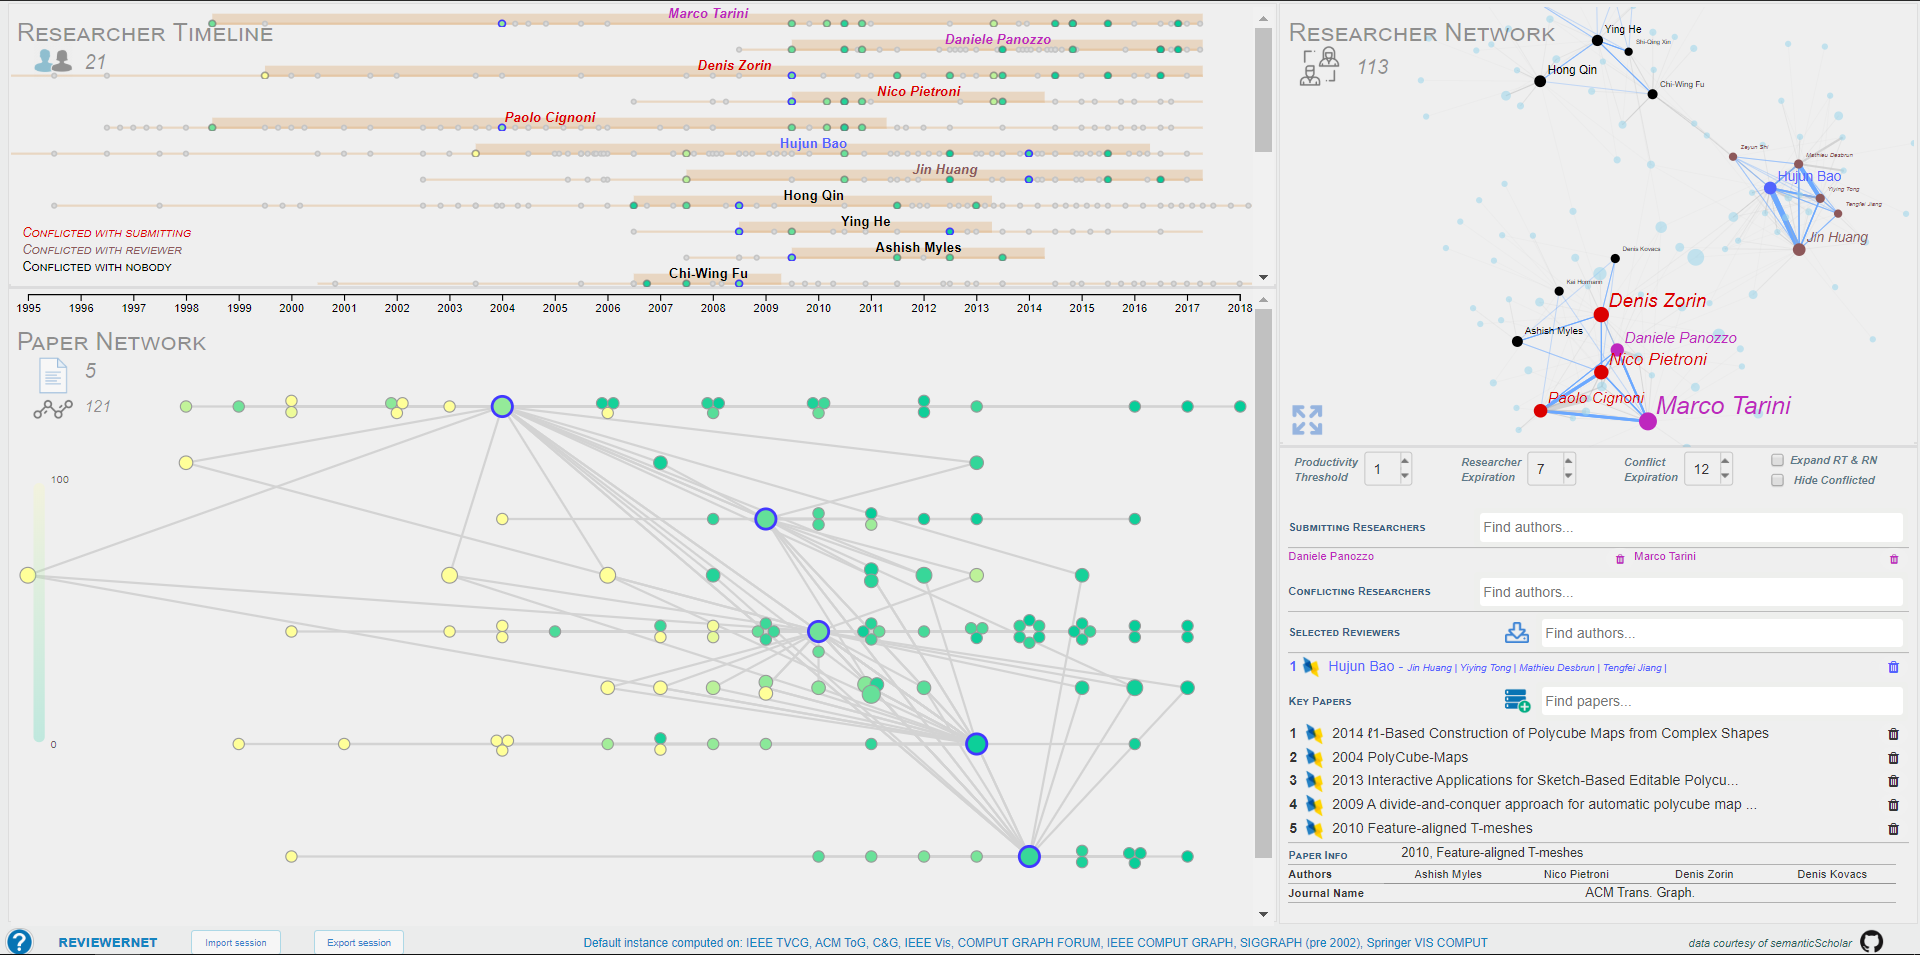
\includegraphics[width=\textwidth]{fig/teaser.png}
    \caption{ReviewerNet user-interface.}%When hovering over an entity representing a paper, the authors of that paper are highlighted in the other views.}
    \label{fig:interface1}
\end{figure*}

Then, the visual composition of the four regions in the interface (Figure~\ref{fig:interface1}) helps the user to gain different perspectives on the problem at hand, within a single visualization. Each region can be resized in height; the Researcher Network can be made full-screen, as in Figure \ref{fig:communities}, for better visualization and interaction.

The nodes in the Paper Network (PN), at the bottom-left hand side of the screen, represent papers in $\mathcal{P}_{V}$, while the arcs represent in- and out-citation relations between them. Apart from pathological cases, the network is by definition a DAG (Directed Acyclic Graph). The visualization of the DAG is constrained along the horizontal direction, since papers are ordered horizontally according to their publication year. While in the previous platform version \cite{stag19} a force-directed graph drawing algorithm determined the layout in the vertical direction \cite{D3js11}, in the new version we preferred a visualization which puts focus on nodes with degree higher than one, that is, on papers which cite/are cited by more than one selected paper. Those papers are are likely to represent relevant papers in the field, and therefore good candidates for being selected as key papers and expanded in the network. Therefore, each key paper is assigned a rectangular region of predefined vertical height; all its citing/cited papers with node degree equal to one are arranged inside the rectangle, whereas nodes with higher degree are positioned in-between the rectangular regions. Their positions minimize the sum of distances from the citing/cited selected papers. This visualization of the network enables one to easily detect higher-degree nodes and network cliques, and tell apart relevant papers, which are good candidates for node selection and expansion. 

Each line in the Researcher Timeline (RT), at the upper-left side of the screen, represents a candidate reviewer $r$ in $\mathcal{R}_{C}$, that is, the author of a selected paper in $\mathcal{P}_{S}$. The dots over the line represent the set $\mathcal{P}|_{r}$ of papers authored by $r$ in the reference database $\mathcal{P}$. %The Researcher Timeline is constructed and updated automatically by ReviewerNet while the user builds and refines the Paper Network.  

The nodes in the Researcher Network (RN), at the upper-right hand side of the screen, are the researchers in $\mathcal{R}_V$ along with their collaborators in $\mathcal{R}$. The arcs connect authors who have publications in common: for each node representing a researcher $r$, the node degree is the cardinality $\vert \mathcal{CA}(r) \vert$. A force-directed graph drawing algorithm determines the graph layout, so that authors who have a large number of publications in common tend to be close to each other. Both the Researcher Timeline and the Researcher Network are built automatically by ReviewerNet while the user builds the Paper Network.  

The Control Panel (CP), at the bottom-right hand side of the screen, allows the user to input and manage the names of submitting authors, the names of selected reviewers, and the titles of key papers. The CP area also displays information about papers, upon request. The DBLP icon beside reviewers' names and paper titles links to their respective DBLP page. Moreover, the CP includes parameters boxes and check-boxes to fine-tune the visualization:

\noindent{\bf Size of data visualized:} 
To limit the number of candidate reviewers visualized in the RT and the RN, the user can set two thresholds a researcher has to meet to be considered as a candidate reviewer: 
\begin{itemize}
\item \emph{Productivity threshold}: the minimum number of authored selected papers in $\mathcal{P}_S$ (i.e., $\vert \mathcal{P}_{S}|_{r} \vert$ has to be greater than the threshold, for a researcher $r$ to be included in the set $\mathcal{R}_C$ of candidate reviewers);
\item \emph{Researcher expiration}: the maximum number of years since the last authored paper in the reference dataset $\mathcal{P}$ (i.e., the number of years has to be lower than the threshold for a researcher to be considered active and included in $\mathcal{R}_C$).
\end{itemize}
The user can also remove conflicting authors and their co-authors from the visualization, by ticking the \emph{Hide Conflicted} checkbox.
To augment instead the number of potential reviewers visualized, the user can tick the \emph{Expand RT \& RN} checkbox: the visualization will include all the researchers in $\mathcal{R}_V$ (all the authors of relevant papers) instead of the researchers in $\mathcal{R}_C$ only (the authors of selected papers only). Note that visualizing a large number of researchers can slow down the interface. \\

\noindent{\bf Conflict-of-interest:} 
Finally, to modulate the conflict of interest, the user can set a threshold for two researchers to be considered as co-authors, namely 
\begin{itemize}
\item \emph{Conflict expiration}: the maximum number of years since the last co-authored paper in $\mathcal{P}$. 
\end{itemize}
A larger threshold will increase the number of candidates marked as conflicted. Conversely, a smaller threshold will increase the number of available reviewers. 

\subsection{Visual consistency}
\label{subsec:visualvar}

Visual cues include the position, colour, size, boundary, and style of visual elements representing papers, researchers and their relations across the different views.  

%\noindent{\bf Visual cues for papers}
\paragraph*{Visual cues for papers} 
For a paper $p \in \mathcal{P}_{V}$, the color may correspond either to the citation count $c(p)$ -- from yellow (few citations) to green (many citations) -- or to the venue where it is published -- according to the eight-value color scale in \cite{Wa13} for the most relevant venues, plus grey for the others; the relevance of a venue is given by its number of incoming citations in the dataset. The colormap applies to both nodes in the PN and dots in the RT. Dots corresponding to papers in $\mathcal{P} - \mathcal{P}_V$ (papers in the reference database, but not included the PN) are marked as grey. 
Selected papers in $\mathcal{P}_S$ are circled in blue, both in the PN and the RT.  Arcs are blue in the RN when the co-authored papers include a selected paper.  

\paragraph*{Visual cues for researchers} 
For researchers in the RT, the name colouring emphasizes the distinction between roles: submitting authors (marked as purple), their co-authors (red), selected reviewers (blue), their co-authors (brown), and non-conflicting, candidate reviewers (black). The nodes in the RN corresponding to researchers in the RT follow the same rule, whereas nodes representing their co-authors in $\mathcal{R}$ are light blue and have no name labels attached.   
For researchers in the RT, the font style of names further helps to tell apart conflicting researchers (italic) from non-conflicting candidate reviewers (normal). The same colour/font rules apply to the names suggested in the selected reviewers' drop-down menu in the CP.
The candidate reviewers in the RT are ordered vertically according to their relevance score (Figure \ref{fig:selected}). The same score is rendered in the RN through the dimension of nodes.  

\subsection{Actions}
\label{subsec:actions}

Each view (PN, RT, RN, CP) is linked to the other views, so that any action in a view is reflected in the others. The shortcut key $Ctrl+Z$ enables the user to undo an action.

\paragraph*{Actions on Papers} 
The user initialises the Paper Network with small set of seed papers. The user can either type the titles of the seed papers in the \emph{Key papers} field, with the help of title-based suggestions, or press the \emph{Import from bibliography} button and paste a list of references. The references are parsed to identify matching titles in the dataset through a fuzzy search; the candidate titles with higher scores are shown to the user, who can select or discard them. Then, the seed papers are visualized in the PN, along with their in- and out-citations. The user can now expand the network, to discover additional documents. With a double click, he selects interesting nodes, i.e., papers he/she deems relevant to the submission topic. The PN then updates with the in- and out-citations of the selected papers. 

Papers can be deselected either with a double click or through the trash bin icon in the Control Panel. 

When the users focuses on a paper in one of the views by mouse hovering, the same paper is highlighted in the other views. For example, when hovering the mouse over a node in the PN, the corresponding dot in the Researcher Timeline is highlighted, and vice-versa. Also, the paper details (title, publication year, venue) are shown in the Control Panel on a mouse click. Likewise, by hovering over or clicking on the title in the CP, the corresponding node and dot are highlighted in the PN and the RT. When hovering the mouse over an entity representing a paper (a node in the PN, a dot in the RT bars, the title in the CP), the paper authors are highlighted in the RT and RN, if present (Figure \ref{fig:overpaper}). A mouse click on the focused paper lets the user navigate the visualization with highlighted items. A single click restores the previous visualization.
The icon beside paper titles in the Control Panel links to DBLP pages. 

\paragraph*{Actions on Researchers} In a similar fashion to papers, when the user focuses on a researcher in one of the views by mouse hovering, the same researcher is highlighted in the other views. When hovering the mouse over a node in the Researcher Network, the name of the corresponding researcher appears on the upper-right corner.  
When hovering the mouse over an entity representing a researcher (a bar in the RT, a dot in the RN, the name in the CP), the papers authored by the researcher are highlighted in the Paper Network view. 
In Figure \ref{fig:authorclick}, a mouse click on a researcher puts the focus on him/her, his/her production and his/her personal net of collaborators. 

The user can navigate a visualization with selected items and additional functionalities. Only the set of co-authors is visualized in the Researcher Timeline and the Researcher Network. While hovering on one of the co-authors, the common publications are shown in the PN, and the arc representing the co-authorship relation is visualized in the RN. Another mouse click will get the user back the previous visualization.
When hovering the mouse over an arc in the RT, like in Figure \ref{fig:researchernetwork}, a pop-up on the upper-right corner shows the pair of co-authors names, the number of common papers in the dataset $\mathcal{P}$, and the number of common relevant papers in $\mathcal{P}_{V}$. In turn, for blue arcs, the common papers are highlighted in the PN. 

\begin{figure*}[!ht]
    \centering
    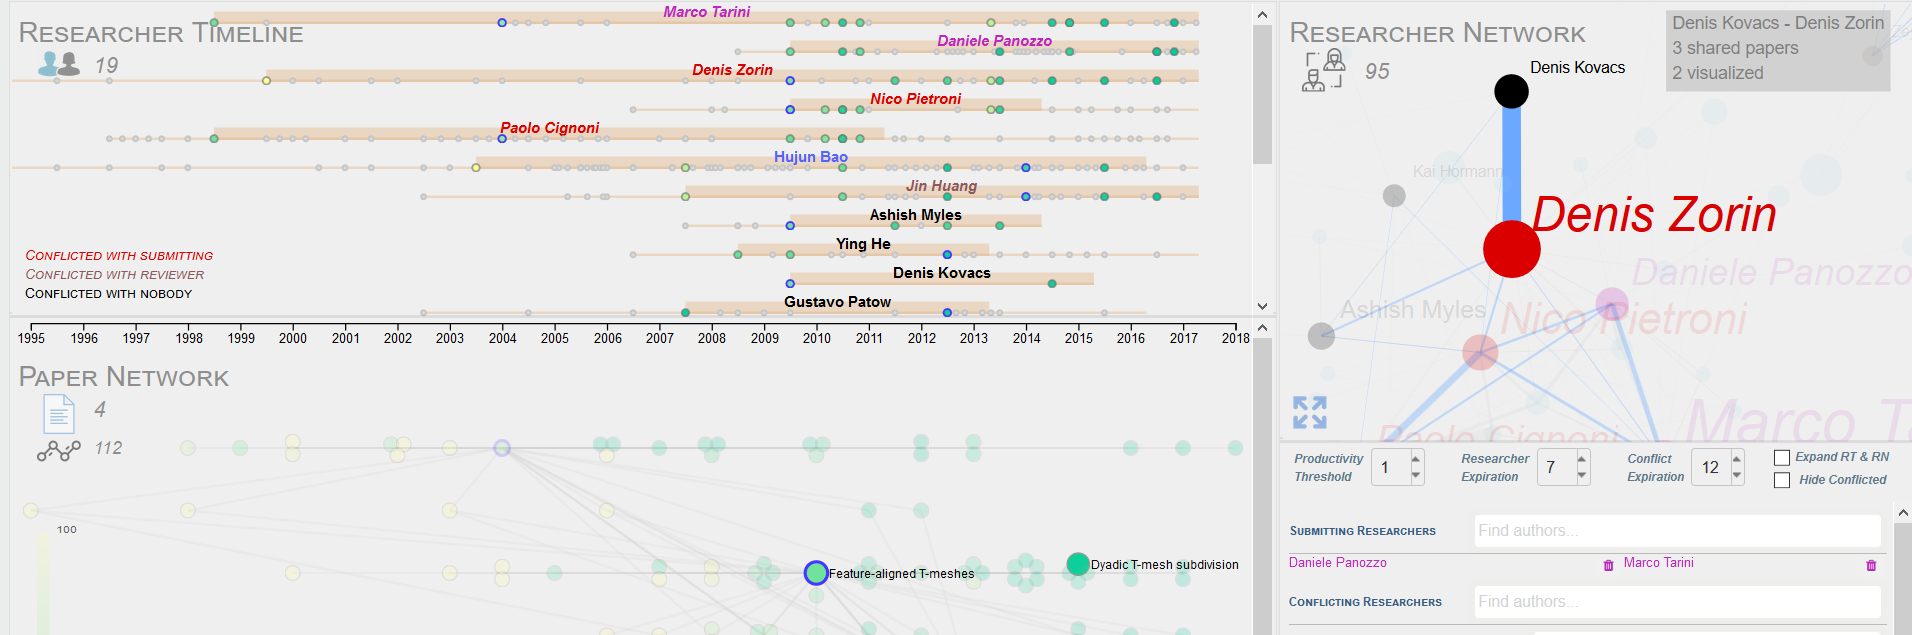
\includegraphics[width=\textwidth]{fig/researchernetwork.png}
    \caption{Hovering over a segment joining two researchers in the Researcher Network shows details about their co-authored papers and highlights them in the Paper Network.}
    \label{fig:researchernetwork}
\end{figure*}

The icon beside the researcher name in any of the fields in the Control Panel links to the DBLP page of that researcher. 
A researcher can be removed from the list of selected reviewers either with a double click or through the trash bin icon in the Control Panel. The user can exchange a reviewer with one of his/her substitutes by clicking on the name of the substitute.
The export button enables the user to download the list of reviewers and their potential substitutes. Work sessions can be saved for later re-use and re-assessment. 
	
	\chapter{Implementation}
\label{sec:impl}
Reviewernet is a fully client-side application. It builds on a bibliographic dataset extracted from a reference corpus containing more than 180 million records.

The goal is to facilitate a complex process, as the reviewer selection, through multiple and coordinated views about papers and researchers.

In this chapter, we describe our implementation choices, namely: the data and the preprocessing phase, languages, frameworks and external libraries used to deploy the user interface, concluding with an analysis of the code that implements additional features of our interactive visualization system.
\section{The data}
To construct the reference dataset, we collected papers, authors and citations from eight selected sources in the field of Computer Graphics, taken from the Semantic Scholar Research Corpus \cite{ammar:18}. 

The original corpus currently contains more than 180 millions research papers published in all fields, provided as a set of gzipped JSON archives. In Figure \ref{jsonfields} there is the full list of the attributes of a generic record that represents a pubblication.

\begin{figure}[!ht]
    \centering
    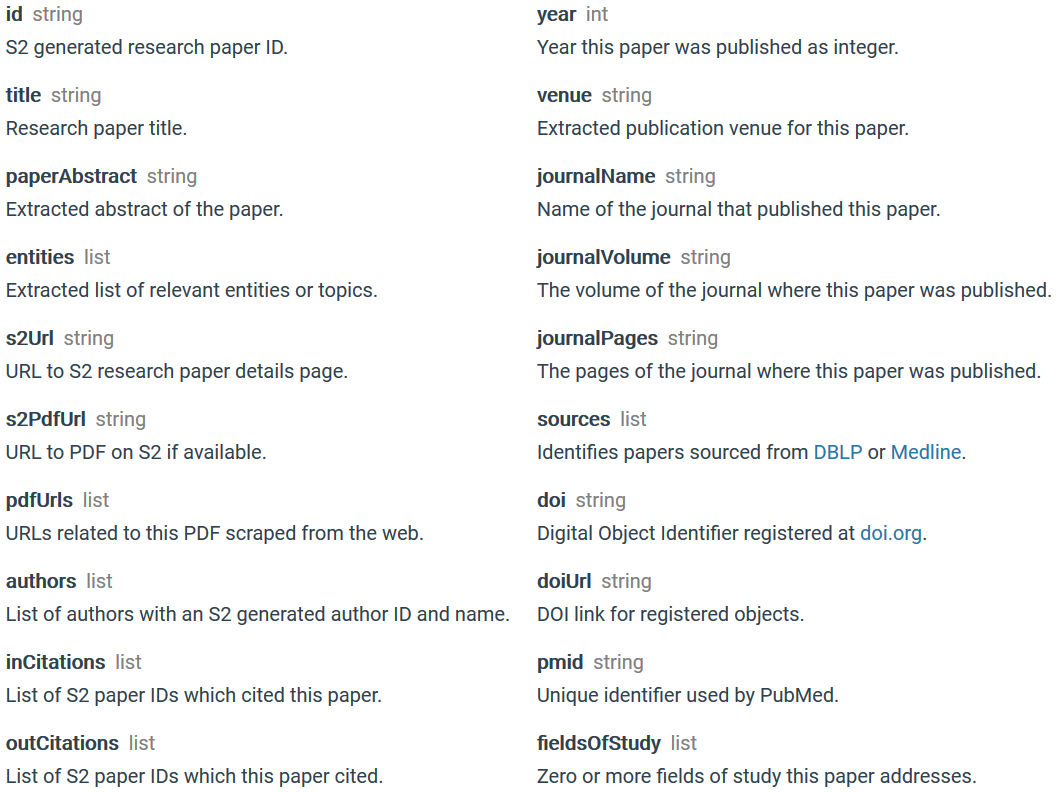
\includegraphics[height=10cm]{fig/corpusfields.png}
    \caption{Definition of attributes of the Semantic Scholar coprus.\label{jsonfields}}
\end{figure}

To keep complexity low and offer a cleaner visualization, we filtered the corpus extracting only publications from journals and conference proceedings listed in Table \ref{table:sources}, spanning the years in-between 1995 and 2019. 

The final reference dataset contains 22.887 papers, 145.900 citations, and 29.549 authors.
\begin{table}[!h]
\renewcommand{\arraystretch}{1.3}
\centering
\begin{tabular}{|l|c|}
\hline
ACM Transactions on Graphics & 2594\\ 
Computer Graphics and Applications  & 1697 \\ 
Computer Graphics Forum & 3521\\ 
Computers \& Graphics & 2092\\ 
IEEE Transactions on Visualization and Computer Graphics & 3638\\ 
Visual Computer & 2107\\ 
Proceedings of IEEE Conference Visualization (pre 2006) & 474 \\ 
Proceedings of ACM SIGGRAPH (pre 2003) & 6718\\
\hline
\end{tabular}
\caption{The selected sources from the Semantic Scholar Research Corpus used in our demonstration scenario. The final reference dataset contains 22.887 papers, 145.900 citations, and 29.549 authors.}
\label{table:sources}
\end{table}

%\input{stats.tex}
\subsection*{Pre-processing}
\label{sec:preproc}

pre-proc is crucial: we want to lower data complexity, while maintaning choerence and topic coverage to properly support the reviewer selection process. After non-paper and useless attributes deletion, each partition parsed and filtered separatedly by a python script. Then consolidation step 
\begin{itemize}
    \item check citations consistency
    \item merge data obtaining 3 files that represent the Computer Graphic reference corpus. (descrivo i tre file con attributi)
\end{itemize}

\section{Languages \& external libraries}
\label{sec:lang}
\begin{itemize}
    \item static UI: HTML5, CSS3, bootstrap
    \item dynamic: JS (JqueryUI for widgets) and D3JS
    \item preproc: Bash and Python (fuzzywuzzy) 
\end{itemize}

\section{Additional features}
\label{sec:misccode}

\begin{itemize}
    \item export/load session snapshot (formato file, spiegare inconsistenza fra id di varie versioni del corpus)
    \item import from biblio \& \texttt{p\_search}
    \item generating a custom reviewernet instance
\end{itemize}

    % !TEX root = main.tex
\chapter{Demonstration}\label{sec:demonstration}
To better explain how ReviewerNet works and supports the reviewer selection process, this section presents an example user scenario. We introduce Robert, a fictitious academic researcher. Robert is in the IPC of a conference in the field of Computer Graphics; he is the primary reviewer for a paper, and he is in charge of finding three additional reviewers, plus alternative reviewers in case of decline. 

Below we describe Robert's interaction with ReviewerNet. In addition, since a static description may not adequately convey the dynamic nature of Robert's investigation, we refer the reader to the accompanying video at \url{https://www.youtube.com/watch?v=JnomPO8QI28}, which illustrates the scenario described below. 

The demonstration platform is available at \url{https://reviewernet.org/}.  

\section{Data collection}

To construct the reference dataset for this scenario, we collected papers, authors and citations from eight selected sources in the field of Computer Graphics, taken from the Semantic Scholar Research Corpus \cite{ammar:18}. The dataset includes data from the journals and conference proceedings listed in Table \ref{table:sources}, spanning the years in-between 1995 and 2018. After an automatic cleaning steps to remove non-papers (such as acknowledgments to reviewers, prefaces, etc.), the final reference dataset contains 17.754 papers, 108.155 citations, and 23386 authors. 

\begin{table}[!t]
\renewcommand{\arraystretch}{1.3}
\centering
\begin{tabular}{|l|c|}
\hline
ACM Transactions on Graphics & 2833\\ 
Computer Graphics and Applications  & 1983 \\ 
Computer Graphics Forum & 3238\\ 
Computers \& Graphics & 2155\\ 
IEEE Transactions on Visualization and Computer Graphics & 3236\\ 
Visual Computer & 2107\\ 
Proceedings of IEEE Conference Visualization (pre 2006) & 501 \\ 
Proceedings of ACM SIGGRAPH (pre 2003) & 1701\\
\hline
\end{tabular}
\caption{The selected sources from the Semantic Scholar Research Corpus used in our demonstration scenario. The final reference dataset contains 17.754 papers, 108.155 citations, and 23386 authors.}
\label{table:sources}
\end{table}


%\input{stats.tex}

\section{ReviewerNet in action}

Robert is in charge of finding reviewers for a paper about polycube maps, authored by Marco Tarini and Daniele Panozzo. He inputs thir names in the \emph{Submitting Authors} field (also with the help of the drop-down menu), and ticks the \emph{Done} checkbox. The authors are now shown in the Researcher Timeline and the Reviewer Network, marked as purple, and the rest of the interface becomes active. 

\subsection{Building the Paper Network} 
\label{sec:demoPN}
The first step is to build the Paper Network, that is, a set of key papers which are relevant to the submission topic. Later on, Robert will chose his reviewers among the authors of those key papers. Robert thinks of a first set of three documents about polycube maps, which serve as seeds for building the network (\emph{PolyCube-Maps}, 2004; \emph{A divide-and-conquer approach for automatic polycube maps construction}, 2009; \emph{$L_1$-based construction of polycube maps from complex shapes}, 2014). He inputs their titles in the \emph{Key papers} field. His knowledge of the domain helps him in this initial step, though he can also take advantage of title-based suggestions, which are shown in a drop-down menu, listed by publication year. The three papers are now included in the Paper Network, along with their in- and out-citations. 

Robert can now expand the network, to discover additional documents. With a double click, he selects interesting nodes, i.e., papers he deems relevant to polycube maps. The Paper Network then updates with the in- and out-citations of the selected papers, so that Robert can further explore the literature. Robert navigates the network, and decides to reduce its size by deselecting a paper he realizes he is no longer interested in, because its citations suggest it addresses a different topic than the submission. Selected papers are marked with a blue contour circle, both in the Paper Network and the Researcher Network. 

Robert continues until he feels the selected papers and their citations offer a good coverage of the literature about the topic at hand. Robert checks the paper details, including the link to the respective DBLP page, shown in the bottom right corner of the interface. A quick keyword search with \emph{polycube maps} in the \emph{Key papers} field let him notice that there is an important paper he was missing (\emph{Efficient volumetric poly-cube map construction}, 2016); the paper can be easily told apart from papers already in the network, thanks to visual cues in the drop-down menu. 

While Robert builds his Paper Network, ReviewerNet automatically adds the authors of selected papers in the Researcher Timeline and the Researcher Network, as candidate reviewers.  The selection of 6 papers produces a list of 28 candidate reviewers. 


\subsection{Exploring the Researcher Timeline and the Researcher Network} 
 
Robert now explores the Researcher Timeline to assess the suitability of candidate reviewers. In the Researcher Timeline, researchers are represented as horizontal lines, spanning their academic career. Robert checks the expertise of candidate reviewers by looking at their stage of career, and production over years. Since each view is linked to the other views, Robert checks topic coverage by looking at who published what, by hovering the mouse over papers to highlight their authors in all the views. He checks conflicts with the submitting authors, thanks to colours and font style. 

The visualization also help Robert analysing the network of collaborators of candidate reviewers. This is fundamental to find sets of independent, well distributed reviewers. With a mouse click on a researcher, ReviewerNet highlights his/her co-authors, and highlights on demand the common publications. Robert further investigates on the collaborations among candidate reviewers by navigating the Researcher Network, a graph visualization of co-authorship relations among the candidate reviewers and their collaborators in the dataset. Robert pans and zooms and uses the different handlers available to discover the communities of collaborators. He founds that there are four distinct groups of collaborators dealing with the topic at hand.

\subsection{Selecting reviewers} 

Once Robert identifies one or more candidate reviewers who fit his requirements, he inputs their names in the \emph{Selected Reviewers} field (also with the help of the drop-down menu). He first decides to chose Pierre Paulin, a senior researcher. The colouring of the selected reviewer switches to blue both in the Researcher Timeline and the Researcher Network, and the colouring of his co-authors switches to grey, to identify them as conflicting potential reviewers, and tell them apart from the remaining available candidates. Then, Robert evaluates Hujun Bao, whose expertise fits with his requirements, then he decides to go for a younger researcher, and selects one of Bao's younger collaborators, Jin Huang. Among the remaining candidates, Robert chooses Xiao-Ming Fu, because he belongs to a different community than the previous two, and he has been working very recently on the subject at hand. 

Robert downloads his list of three reviewers with a click on the download button. The list reports reviewers' names and bibliographic references to their papers. 

After contacting the reviewers, Robert finds that one of them declines his invitation. Fortunately, for each reviewer selected by Robert, ReviewerNet has automatically added a list of potential alternative reviewers, in case of a negative answer by the original reviewer. Alternative reviewers are chosen from the candidate ones, so that they only conflict with the declining reviewer. Robert evaluates possible substitutes, again taking advantage of ReviewerNet functionalities, and finds his best replacement.  

\subsection{Discussion} 

This abreviated scenario shows how ReviewerNet can support investigating the literature, learning who are the experts in a field, and exploring relationships among them. The description above necessarily simplified a typical intercation process: Robert could of course switch back and forth between different tasks. For example, he could have refined the Paper Network after having examined the list of candidate reviewers. He could have adjusted the size of the list by fine tuning the parameters defining the criteria on productivity to be included in the list, or the criteria that defined conflicts. The process is iterative in nature, and the desiderata may evolve as the search proceeds. Thanks to the user-friendly interface which leaves the user control over the process, ReviewerNet enables the user to narrow down as well as widen the scope of analysis. In turn, the combined visualization of different aspects of the problem at hand well supports the decision making process.     


    
    % !TEX root = main.tex
\chapter{Evaluation}\label{sec:evaluation}

We evaluated the preliminary version of ReviewerNet described in \cite{stag19} on the dataset focused on Computer Graphics described in Chapter \ref{sec:demonstration}. We decided to ask the scientific community directly, and involve real end-users instead of in-house testers. We sent an email to the 60 members of the IPC of Eurographics Conference 2019, and to additional experts with a record of publications in the top venues of the sector. None of the subjects were involved in the work on ReviewerNet, and none of them knew the system prior to the evaluation test. The participation was on a volunteer basis, with no reward.

We collected 7 responses from the IPC members (10\% of the IPC) and 8 responses from additional experts for a total of 15 users. The questionnaire was anonymous and the volunteers were asked to answer three questions about themselves: number of years from their PhD, reviews and reviewer selections per year; Table \ref{table:infotesters} shows the distribution of the results of this part of the questionnaire

\begin{table}[!t]
	\renewcommand{\arraystretch}{1.3}
	\caption{Information about the 15 participants in the user study.}
	\label{table:infotesters}
	\begin{subtable}[t]{.99\linewidth}
		\centering%
		\begin{tabular}{|p{3cm}|c|c|c|}
			\hline
			\ & PhD & $\leq$ 12 & $>$ 12\\
			\hline
			{\bf Years from PhD} & 0.0\% & 66.7\% &  33.3\% \\
			\hline
		\end{tabular}
  \end{subtable}
	\par\bigskip
  \begin{subtable}[t]{.99\linewidth}
		\centering
		\begin{tabular}{|p{3.9cm}|c|c|c|}
			\hline
			\ & $<$ 10 & 10 - 20 & $>$ 20\\
			\hline
			{\bf Reviews per year} & 6.7\% & 40.0\% &  53.3\% \\
			\hline
		\end{tabular}
  \end{subtable}
	\par\bigskip
  \begin{subtable}[t]{.99\linewidth}
		\centering
		\begin{tabular}{|p{5.15cm}|c|c|}
			\hline
			\ & $\leq$ 3 & $>$ 3\\
			\hline
			{\bf Reviewer selections in 2018} & 13.3\% &  86.7\% \\
			\hline
		\end{tabular}
  \end{subtable}
\end{table}

%The members of the EG IPC were asked to search three reviewers with ReviewerNet, for one of the EG submissions they had searched reviewers for. 
The volunteers were asked to search three reviewers for a paper that they had to choose reviewers for in the recent past. This was done so that we could not only collect feedback on the system itself, but also enable the volunteers to comparatively evaluate the performance of the system.

For training, the volunteers were only provided with a 6-minutes video demonstrating the usage of ReviewerNet, namely the video recording a similar scenario to Chapter \ref{sec:demonstration}. We did not give any additional training. Also, we asked for a response within five days. This was done to evaluate whether it was easy to get acquainted with ReviewerNet, and whether the system was intuitive and quick to learn. Only one user out of 15 (6.7\% of the sample) reported s/he was not able to figure out how to use the system. 

The other 14 (93.3\%) were able to complete the task assigned with the little support offered. This confirms the user-friendliness of the instrument even if the tool offers many different interaction modalities.

The rest of the questionnaire was divided in two sections, whose questions and summary of answers are reported in Table \ref{table:formsection1} and Table \ref{table:formsection2}, respectively. The first section asked the user's opinion about the different functionalities of ReviewerNet, namely: finding key papers (and hence key researchers); presenting the scientific career of candidate reviewers; avoiding conflicts of interest; and finding sets of well distributed reviewers:% The possible answers followed a five-point scale from \emph{Very poor} to \emph{Excellent}. Table \ref{table:formsection1} summarizes the results for this section:
\begin{itemize}
\item [73.3\%] of the testers evaluated ReviewerNet as either good or excellent in finding key papers and researchers. 
\item [80.0\%] of the testers evaluated as good or excellent the presentation of the scientific career of candidate reviewers. One of the testers found that {\em "[...] the timeline also is a great added value with respect to imagining whether an author is doing a similar research now or he did many years ago"};
\item [ 86.7\%] of the testers thought ReviewerNet was good or excellent to help avoiding conflicts of interest. One of the testers observed how {\em "[...] the tool actually follows my current practice, that is, look among authors of key papers"} but with the added value of the explicit labelling of conflicting reviewers. He/she also observed that {\em "[...] the labelling of conflicting reviewers helps also a lot. [...] the tool also helps in selecting reviewers from different areas, covering better the topic of a paper."}
\item [ 66.7\%] evaluated as good or excellent ReviewerNet support to find sets of well distributed reviewers. 
\end{itemize}

The second section of the questionnaire asked the users an overall opinion on ReviewerNet, in terms of improvement of the overall quality of the reviewing process, and reduction in the time spent to search for reviewers:  % The possible answers followed a five-point scale from \emph{Strongly disagree} to \emph{Strongly agree}. %The third part of the questionnaire it required to compare the reviewer selection experience with and without ReviewerNet; this was done so that we could not only collect feedback on the system itself, but also comparative data with respect to the traditional pipeline. This section was for the EG IPC members only: as the request was sent just after the first review cycle had been completed, this made sure that the testers had a recent enough memory of their experience without Reviewernet. The third section asked the users whether searching for reviewers had taken shorter time with ReviewerNet; whether ReviewerNet had proposed good candidate reviewers they had not thought about, or missed candidate reviewers they had in mind; and additional comments. 
%
%Table \ref{table:formsection2} summarizes the results for the second section. 
\begin{itemize}
\item [71.4\%] of the testers agreed or strongly agreed that ReviewerNet helps choosing good sets of reviewers, and hence improves the overall quality of the reviewing process;
\item [71.4\%] agreed or strongly agreed that ReviewerNet reduces the time spent to look for good sets of reviewers. 
\end{itemize}

In addition, the testers could insert additional comments about ReviewerNet strengths and weaknesses, and suggestions for improvement. We used their comments and suggestions to improve on the preliminary version of the platform.

In particular, one of the testers observed that {\em "[...] inserting manually key papers, takes a little more time, but then the system helps a lot navigating trough related papers and authors"}. Therefore, to reduce the burden on users to initialize the Paper Network and the whole system, we added the \emph{Import from bibliography} functionality, which enables the automatic parsing and matching of lists of references pasted from the References section of articles.

One of the testers found  {\em "[...] a little difficult the interpretation of the researchers network on the top/right. The view is a bit complicated, not immediately clear which node corresponds to the clicked reviewer from the bars on the top/left,
[...] but probably again it is just a matter of more practice}". The Researcher Network can be now made full-screen for better visualization and interaction. The nodes are labelled with names, while the node embedding better reflects the closeness of researchers in terms of collaborations (number of co-authored papers). The embedding can be also modified interactively by the user via drag-and-drop.

\begin{table*}[!t]
	\renewcommand{\arraystretch}{1.3}
	\caption{ Distribution of answers to the first section of the questionnaire (14 participants) where the acronyms in the first row stand for: Very poor, Poor, Average, Good and Excellent.}
	\vspace{0.3cm}
	\label{table:formsection1}
    \centering%
		\begin{tabular}{|p{0.4\textwidth}|c|c|c|c|c|}
			\hline
			& VP & P & A & G & E\\
			\hline 
			{{\em How do you rate ReviewerNet in finding key papers and researchers?}}                      & 0.0\% & 0.0\% &  26.7\% & {\bf 46.6\%} & 26.7\% \\
			\hline
			{{\em How do you rate ReviewerNet in presenting the scientific career of candidate reviewers?}} & 0.0\% & 6.7\% &  13.3\% & {\bf 46.6\%} & 33.3\% \\
			\hline
			{{\em How do you rate ReviewerNet in avoiding conflicts of interest?}}                          & 0.0\% & 6.7\% &   6.7\% & 40.0\% & {\bf 46.7\%} \\
			\hline
			{{\em How do you rate ReviewerNet in finding sets of well distributed reviewers?}}              & 0.0\% & 6.7\% &  26.7\% & {\bf 40.0\%} & 26.7\% \\
			\hline
		\end{tabular}
\end{table*}

\begin{table*}[!t]
	\renewcommand{\arraystretch}{1.3}
	\caption{Distribution of answers to the second section of the questionnaire (13 participants) where the acronyms in the first row stand for: Strongly Disagree, Disagree, Neutral, Agree and Strongly agree.}
	\vspace{0.3cm}
	\label{table:formsection2}
    \centering%
		\begin{tabular}{|p{0.4\textwidth}|c|c|c|c|c|}
			\hline
			& SD & D & N & A & SA\\
			\hline 
			{{\em I think that ReviewerNet helps choosing good sets of reviewers, and hence improves the overall quality of the reviewing process}.} & 0.0\% & 0.0\% &  28.6\% & {\bf 35.7\%} & {\bf 35.7\%} \\
			\hline
			{{\em I think that ReviewerNet reduces the time spent to look for good sets of reviewers}.}                                              & 0.0\% & 0.0\% &  28.6\% & 28.6 & {\bf 42.9} \\
			\hline 
		\end{tabular}
	\par
\end{table*}

Concerning ReviewerNet ability to find key papers and researchers, one of the testers observed that vision-related venues (e.g., conferences such as CVPR and ICCV and journal such as IJCV and TPAMI) were missing from the list of sources for key papers and authors on which the demonstration tool was built. He/she observed that the tool would have been more useful if these were included, since many works overlap vision and graphics. Similarly, another tester observed that the homogeneous nature of the sources selected made so the proposed reviewers could show no enough divergence and could be scarce. In this respect, it is worth noticing that ReviewerNet can be built over \emph{any} subset of the Semantic Scholar corpus and customized to include the venues of interest. Therefore, these comments mostly apply to the particular instance used for testing. The version of the platform presented in this thesis features the possibility to upload a personalized list of venues, pertaining to any academic domain, and on which to build a customized dataset. %, rather than to the platform per se. 


We believe the results from the evaluation study showed a very high value of user satisfaction, and also offered useful suggestions for improvement.




  




   

      
    
    % !TEX root = cag-reviewernet.tex

\chapter{Conclusions}
\label{sec:conclusions}

We have presented ReviewerNet, a novel system for choosing reviewers by visually exploring scholarly data. ReviewerNet enables scientific journal editors and members of IPCs to search the literature about the topic of a submitted paper, to identify experts in the field and evaluate their stage of career, and to check possible connections with the submitting authors and among the reviewers themselves. This helps to avoid conflicts and to build a fairly distributed pool of reviewers. To do so, ReviewerNet features a combined visualization of the literature, the career of potential reviewers, their conflict of interests, and their nets of collaborators. Interestingly enough, the system is able to help the process even without exploiting any content-based analysis of the papers.

%The results from a user study involving 15 senior members from the Computer Graphics community confirmed that they were able to get acquainted with the system even with a very limited training, and  appreciated the different functionalities of ReviewerNet and its capability of improving the reviewer search process.

\textcolor{red}{The evaluation of a preliminary version of the demonstration platform} with both in-house testers and members from the Computer Graphics community confirmed that the users were able to get acquainted with the system even with a very limited training, and  appreciated the different functionalities of ReviewerNet and its capability of improving the reviewer search process.  
Some of the users also highlighted the potential of ReviewerNet as a tool to support bibliographic research, besides the reviewer selection process. 

The evaluation also highlighted \textcolor{red}{that there was room for improving the system, which we did by: improving on the effectiveness of the visualization and the user-friendliness of the interaction modes; improving the initial process of selecting key papers, whose manual insertion was signalled as a weakness by some users, by importing the bibliography of papers; defining a procedure to generate instances of the platform with customizable data coverage, by loading one's own reference dataset. Additional directions for improvement include: an automatic strategy to suggest key papers by computing network features (e.g., betweenness  centrality); and a user-friendly visual interface for building the reference dataset, through the assisted selection a list of venues of interest.}    

\textcolor{red}{Also, we are currently planning to carry out a second formal user study with end users on the revised platform, to assess both the individual visualization design strategies, and the overall system usability and performance.} 

%, in its current state ReviewerNet focuses on the deterministically mechanical part of the process, minimizing the possibility of introducing any bias in the process. 
%We also plan to discuss with providers of scholarly data about the possible release of a version of ReviewerNet with customizable data coverage, to be used by the various scientific communities.  


    
    \chapter*{Acknowledgments}

The authors would like to thanks the Allen Institute for Artificial Intelligence for providing the Semantic Scholar corpus of bibliographic data.


%    \chapter*{Ringraziamenti}
------------   
\newpage
\bibliography{ReviewerNetBib}
\bibliographystyle{IEEEtran}
%    \begin{thebibliography}{}
\bibitem{stat1} 
L. Martinelli e L. Baldini,
\textit{Misure ed analisi dei dati: introduzione al laboratorio di fisica}. 
Edizioni ETS, 4a ed Settembre 2009.
\bibitem{stat2} 
R. Giuliano, \textit{Argomenti di probabilità e statistica}. Springer, 2011.
\bibitem{sec} 
S. Katzenbeisser e F. Petitcolas, \textit{Defining Security in Steganographic Systems}, in \textit{Proceedings of SPIE}, \textit{Security and Watermarking of Multimedia Contents IV}. International Society for Optical Engineering, 2002, pp. 50-56.
\bibitem{simmons}
G. Simmons, \textit{The Prisoners' Problem and the Subliminal Channel}, in \textit{Advances in Cryptology}. Plenum Press, 1984, pp. 51-67.
\bibitem{approach}
C.Cachin, \textit{An Information-Theoretic Model for Steganography}, in \textit{Information Hiding: Second International Workshop}. vol. 1525, Springer, 1998, pp. 306-318.
\bibitem{zoller}
J. Z\"oller et al., \textit{Modeling the Security of Steganographic Systems}, in \textit{Information Hiding: Second International Workshop}, vol. 1525, Springer, 1998, pp. 306-318.
\bibitem{fried1}
J. Fridrich e M. Goljan, \textit{Practical Steganalysis of digital images – State of the Art}, in \textit{Proceedings of SPIE, Security and Watermarking of Multimedia Contents IV}, International Society for Optical Engineering, 2002, pp. 1-13.
\bibitem{fried2}
J. Fridrich, M. Goljan e R. Du, \textit{Reliable detection of LSB steganography in color and grayscale images}, in \textit{Proceedings of 2001 ACM workshop on Multimedia and Security: new challenges}, ACM press, 2001, pp. 27-30.
\bibitem{chisq}
A.Westfeld e A. Pfitzman, \textit{Attacks on steganographic System. Breaking the Steganographic Utilities EzStego, Jsteg, Steganos and S-Tools and some lessons learned}, in \textit{Proceedings of third International Information Hiding Workshop}, vol. 1768, Springer, 1999, pp. 67-76.
\bibitem{survey}
B. Lin, J. He, J. Huang e Y.Q. Shi, \textit{A survey on image steganography and steganalysis}, in \textit{Journal of Information
Hiding and Multimedia Signal Processing}, vol. 2, no. 2, 2011, pp. 142-172.
\bibitem{survey2}
Y.J. Chanu, Kh.M. Singh e T. Tuithung, \textit{Image Steganography and Steganalysis: A Survey}, in \textit{International journal of Computer Applications}, vol. 52, no. 2, 2012.
\bibitem{seeingTheUnseen}
N.F. Johnson e S. Jajodia, \textit{Exploring steganography: seeing the unseen}, in \textit{IEEE Computer}, vol. 31, no. 2, pp. 26-34, 1998.
\bibitem{experts}
T. Aura, \textit{Invisible Communication}, in \textit{Technical report of Helsinki Univ. of Technology}, EET, 1995.
\bibitem{warfare}
H. Wang e S. Wang, \textit{Cyber Warfare: Steganography  vs Steganalysis}, in \textit{Communications of the ACM}, vol. 47, no 10, pp. 76-82, 2004.
\bibitem{provos}
N. Provos, \textit{Defending Against Statistical Steganalysis}, in \textit{10th USENIX Secutiry Symposium}, 2001.
\bibitem{sup}
R. Chandramouli e N. Memon, \textit{Analysis of LSB based Image Steganography Techniques}, in \textit{Proceedings of ICIP}, 2001.
\bibitem{mat1}
J. Mielikainen, \textit{Lsb matching revisited}, in \textit{IEEE Signal Processing Letters}, vol. 13, no. 5, pp. 285-287,
2006.
\bibitem{mat2}
X. Li, B. Yang, D. Cheng, e T. Zeng, \textit{A generalization of lsb matching}, in \textit{IEEE Signal Processing
Letters}, vol. 16, no. 2, pp. 69-72, 2009.
\bibitem{sito}
ESET Research, \textit{Readers of popular websites targeted by stealthy Stegano exploit kit hiding in pixels of malicious ads}, in \textit{ESET Research Papers}, 2016.
\bibitem{improved}
X. Luo, B. Liu e F. Liu, \textit{Improved RS method for detection of LSB steganography}, in \textit{Computational Science and Its Applications -- ICCSA 2005: International Conference, Singapore, Proceedings}, Springer Berlin Heidelberg, 2005, pp. 508-516.
\end{thebibliography}
\end{document}
